%%%%%%%%%%%%%%%%%%%%%%%%%%%%%%%%%%%%%%%%
%                                      %
%   Non usate caratteri piu' piccoli   %
%                                      %
%%%%%%%%%%%%%%%%%%%%%%%%%%%%%%%%%%%%%%%%

\documentclass[12pt]{article}
\usepackage[latin1]{inputenc}
\usepackage[a4paper]{geometry}
\usepackage{graphicx}
\usepackage{amsmath} 
\usepackage{amssymb} 
\usepackage{makeidx}

% inserite ovviamente tutti i package che volete usare

\topmargin -1cm
\oddsidemargin -0.5cm
\textwidth 16.5cm
\textheight	23.5cm

\newcommand{\Nomecomando}{Testocomando}
\newcommand{\degree}{\ensuremath{^\circ}}

\title{Expansions and Equations}
\date{}
\author{Andrea Caleo, Andrea Mauri}

%\makeindex

\begin{document}
%\maketitle 
%\tableofcontents \break
\section{GS Notes}
GS dispersion relation:
\begin{equation}
q^3 + A(\vec k) q^2 + B(\vec k) q + C(\vec k) = 0
\end{equation}

\begin{equation}
A(\vec k) = \frac{k^2}{\Omega} \Big( 2\nu +  \frac{1}{\gamma} \xi \Big)
\end{equation}

\begin{equation}
B(\vec k) = \Big( \frac{k_z}{k} \Big)^2 \Big[ \frac{1}{\gamma \Omega^2 \rho} (- \tilde D P + \rho \Omega^2 R) \tilde D \sigma -  \frac{2}{\Omega R} \tilde D l \Big] + \frac{2}{\gamma} \Big( \frac{\xi  k^2}{\Omega} \Big)  \Big( \frac{\nu k^2}{\Omega} \Big)
\end{equation}


\begin{equation}
C(\vec k) = \Big( \frac{k_z}{k} \Big)^2 \Big[ \frac{1}{\gamma \Omega^2 \rho} \Big( \frac{\nu k^2}{\Omega} \Big) (- \tilde D P + \rho \Omega^2 R) \tilde D \sigma - \frac{2}{\gamma \Omega R} \Big( \frac{\xi  k^2}{\Omega} \Big)  \tilde D l  \Big] + \frac{1}{\gamma} \Big( \frac{\xi  k^2}{\Omega} \Big) \Big(\frac{\nu k^2}{\Omega} \Big)^2
\end{equation}

\begin{equation}
\tilde D = \frac{k_R}{k_z} \frac{\partial}{\partial z} - \frac{\partial}{\partial R}
\end{equation}

There are unstable modes if $C(\vec k) < 0$. We discard the last term in $C$, which is always positive, and neglect $\rho \Omega^2 R$ compared to $\tilde D P$. The condition $C(\vec k) < 0$ can be rewritten as ($\text{Pr} \equiv  \nu / \xi$):

\begin{equation} \label{eqPr}
\text{Pr} < - \Big( \frac{\Omega r}{c_s} \Big)^2 \frac{2 \gamma}{ ( - \frac{d \log P}{d \log r}) (\frac{d \sigma}{d \log r})} \times \frac{2 + \frac{d \log \Omega}{d \log R} - x \tan{\theta} \frac{d \log \Omega}{d \log z}}{ (x \cos \theta - \sin \theta)^2}   , 
\end{equation}
where $c_s^2 = \gamma P/\rho$, $\sigma = \log (P \rho^{-\gamma})$. Typical values at $r = 0.6 R_\odot$:
\begin{equation}
\Big( \frac{\Omega r}{c_s} \Big)^2 \sim 2 \cdot 10^{-5}, \qquad \frac{d \log P}{d \log r} \sim -6.9, \qquad \frac{d \log \sigma}{d \log r} \sim 2.6,
\end{equation}
\begin{equation}
  \qquad \frac{d \log \Omega}{d \log R} \sim -0.001, \qquad \frac{d \log \Omega}{d \log z} \sim -0.02 .
\end{equation}
At $r = 0.7 R_\odot$, the logarithmic derivatives of $P$ and $\sigma$ are only moderately different, while those of $\Omega$ are larger by an order of magnitude.

We note that the numerical factor $2 \gamma / \Big[  ( - \frac{d \log P}{d \log r}) (\frac{d \sigma}{d \log r}) \Big]$ is therefore positive and of order unity or less. For mid-latitudes, $\tan \theta \frac{d \log \Omega}{d \log z}$ is less than 0.1 and the numerator of the last term is positive. The condition reduces to $\text{Pr} < Q$ with $Q < 0$ which is clearly satisfied for any viscosity. The only cases in which the instability may occur are those for which the numerator of the last term is negative. Unless $\tan \theta$ is large, i.e. $\theta$ is close to $\pi/2$, this implies that $|x| >> 1$.  In this case, however, the denominator of is also large, of order $x^2$, and the term results small overall. We explored the maximum of the function for values of $\theta$ in the $5 - 85 \degree$ and $r = 0.5 R_\odot - 0.7 R_\odot$ and found that it is always well below $\sim 10^{-2}$. We show the maximum of the function:
\begin{equation}
N(x; r, \theta) = \frac{2 \gamma}{ ( - \frac{d \log P}{d \log r}) (\frac{d \sigma}{d \log r})} \times \frac{2 + \frac{d \log \Omega}{d \log R} - x \tan{\theta} \frac{d \log \Omega}{d \log z}}{ (x \cos \theta - \sin \theta)^2} 
\end{equation}
for $- 10^6 < x < 10^6$ as a function of $r$ for 3 values of the co-latitude $\theta$ in figure \ref{figNumFact}.
\begin{figure}
	\centering
	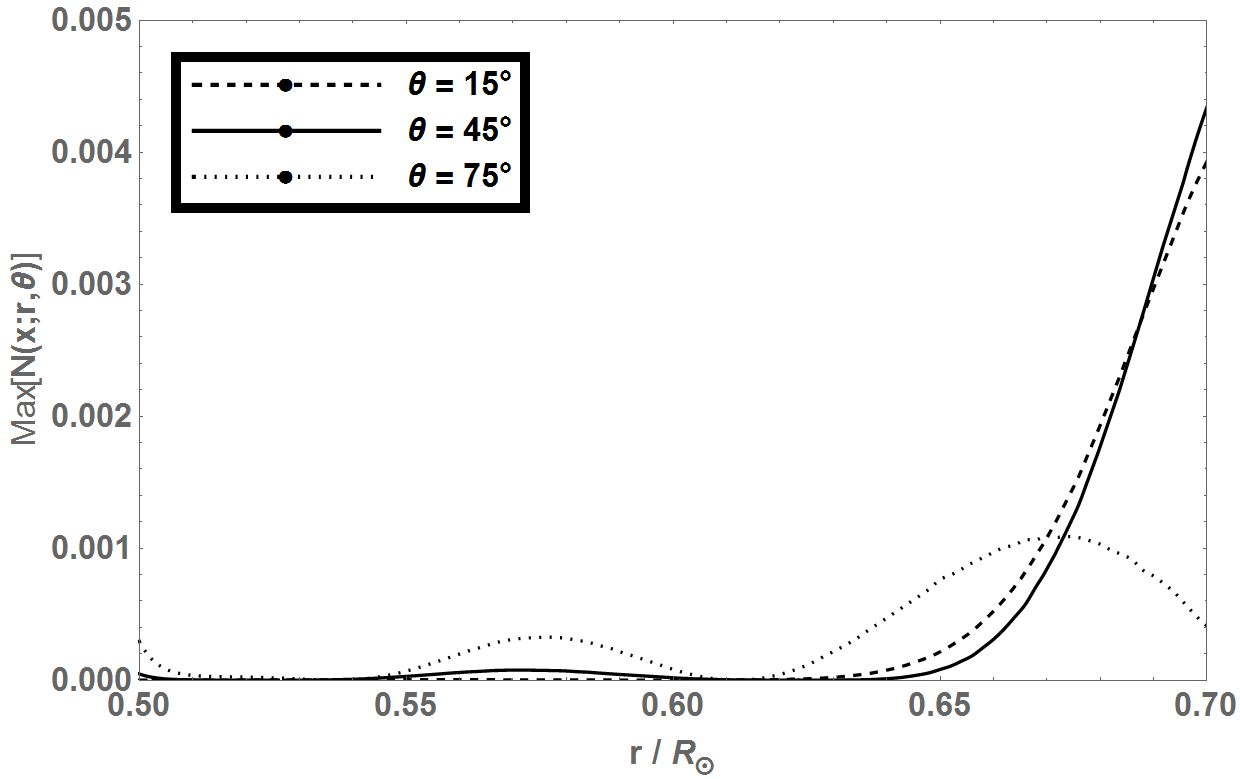
\includegraphics[width=\textwidth, clip=true, trim=0cm 0cm 0cm 0cm]{picNumFact.png}			
	\caption{\label{figNumFact}Maximum of $N(x; r, \theta)$ for $- 10^6 < x < 10^6$.}
\end{figure}

Finally, we explored the maximum of such term for $\theta \rightarrow \pi/2$. We have not found any higher value of it. The reason is as follows: while $\tan \theta \rightarrow + \infty$ for $\theta \rightarrow \pi/2$, it's also true that:
\begin{equation}
\frac{d \log \Omega}{d \log z} = \frac{z}{\Omega} \frac{d \Omega}{dz} \rightarrow 0  \ \text{for} \  \theta \rightarrow \pi/2
\end{equation}

The condition for instability is therefore:
\begin{equation}
\text{Pr} \lesssim 10^{-2} \Big( \frac{\Omega r}{c_s} \Big)^2
\end{equation}
This condition (except for the numerical factor $10^{-2}$) holds as long as $|\frac{d \log \Omega}{d \log R}|$ and $|\frac{d \log \Omega}{d \log z}|$ are smaller than 2. At this point, values of $x \sim 1$ may be sufficient to make the numerator of the last term of \eqref{eqPr} positive where the denominator vanishes, and the system may be unstable even for large values of $\text{Pr}$.

So in general we can say: 
\begin{equation} \label{eqCondition}
\text{Pr} = \frac{\nu}{\xi} \lesssim \Big( \frac{\Omega r}{c_s} \Big)^2
\end{equation}
The viscosity $\nu = \nu_{\text{dyn}} + \nu_\text{rad}$ where $\nu_\text{dyn}$ and $\nu_\text{rad}$ are the dynamical and radiative viscosity respectively. In most cases, $\nu_\text{dyn}$ dominates in a star. However, let's consider the case in which $\nu_\text{rad}$ is significant. It is known that:
\begin{equation}
\text{Pr}_\text{rad} = \frac{\nu_\text{rad}}{\xi} \cong \Big(\frac{c_s}{c}\Big)^2,
\end{equation}
where $c_s$ is the sound speed; see e.g. Mihalas (1983). The condition \eqref{eqCondition} therefore prescribes that the onset of the instability is only possible if:
\begin{equation}
\Omega r \gtrsim c_s \cdot \frac{c_s}{c}
\end{equation}
Typically, in a stellar core, $c_s/c \sim 10^{-3}$; hence the condition is $v_{rot} \gtrsim 10^{-3} c_s$. For example, for the angular velocity with the discontinuity for model D of Deheuvels et al. (2014), this would require $\Omega \gtrsim 9 \times 10^4$ nHz, which is not observed (their fit gives $\Omega \sim 5 \times 10^3$ nHz).



\end{document}























